\documentclass[10pt, letterpaper]{article}

% Packages:
\usepackage[
    ignoreheadfoot,
    top=2 cm,
    bottom=2 cm,
    left=2 cm,
    right=2 cm,
    footskip=1.0 cm,
]{geometry}
\usepackage[explicit]{titlesec}
\usepackage{tabularx}
\usepackage{array}
\usepackage[dvipsnames]{xcolor}
\definecolor{primaryColor}{RGB}{0, 79, 144}
\usepackage{enumitem}
\usepackage{fontawesome5}
\usepackage{graphicx}
\usepackage{amsmath}
\usepackage[
    pdftitle={Leonardo Silvagni's CV},
    pdfauthor={Leonardo Silvagni},
    pdfcreator={LaTeX},
    colorlinks=true,
    urlcolor=black
]{hyperref}
\usepackage[pscoord]{eso-pic}
\usepackage{calc}
\usepackage{bookmark}
\usepackage{lastpage}
\usepackage{changepage}
\usepackage{paracol}
\usepackage{ifthen}
\usepackage{needspace}
\usepackage{iftex}
\usepackage{verbatim}
\usepackage{etoolbox}

\ifPDFTeX
    \input{glyphtounicode}
    \pdfgentounicode=1
    \usepackage[T1]{fontenc}
    \usepackage[utf8]{inputenc}
    \usepackage{lmodern}
\fi

\usepackage[default, type1]{sourcesanspro}

% Footer style:
\AtBeginEnvironment{adjustwidth}{\partopsep0pt}
\pagestyle{empty}
\setcounter{secnumdepth}{0}
\setlength{\parindent}{0pt}
\setlength{\topskip}{0pt}
\setlength{\columnsep}{0.15cm}
\makeatletter
\let\ps@customFooterStyle\ps@plain
\patchcmd{\ps@customFooterStyle}{\thepage}{
    \color{gray}\textit{\small Leonardo Silvagni - Page \thepage{} of \pageref*{LastPage}}
}{}{}
\makeatother
\pagestyle{customFooterStyle}

% Section title format:
\titleformat{\section}{
    \needspace{4\baselineskip}
    \Large\color{primaryColor}
}{}{0pt}{
    \textbf{#1}\hspace{0.15cm}\titlerule[0.8pt]\hspace{-0.1cm}
}[]
\titlespacing{\section}{-1pt}{0.3cm}{0.2cm}

% List environments:
\newenvironment{highlights}{
    \begin{itemize}[
        topsep=0.10 cm,
        parsep=0.10 cm,
        partopsep=0pt,
        itemsep=0pt,
        leftmargin=0.4 cm + 10pt
    ]
}{
    \end{itemize}
}
\newenvironment{highlightsforbulletentries}{
    \begin{itemize}[
        topsep=0.10 cm,
        parsep=0.10 cm,
        partopsep=0pt,
        itemsep=0pt,
        leftmargin=10pt
    ]
}{
    \end{itemize}
}

\newenvironment{onecolentry}{
    \begin{adjustwidth}{0.2 cm + 0.00001 cm}{0.2 cm + 0.00001 cm}
}{
    \end{adjustwidth}
}

\newenvironment{twocolentry}[2][]{
    \onecolentry
    \def\secondColumn{#2}
    \setcolumnwidth{\fill, 4.5 cm}
    \begin{paracol}{2}
}{
    \switchcolumn \raggedleft \secondColumn
    \end{paracol}
    \endonecolentry
}

\newenvironment{threecolentry}[3][]{
    \onecolentry
    \def\thirdColumn{#3}
    \setcolumnwidth{1 cm, \fill, 4.5 cm}
    \begin{paracol}{3}
    {\raggedright #2} \switchcolumn
}{
    \switchcolumn \raggedleft \thirdColumn
    \end{paracol}
    \endonecolentry
}

% --- header environment ---
\newenvironment{header}{%
  % pull whole header upward (adjust to taste)
  \vspace*{-0.6cm}%

  \color{primaryColor}\linespread{1.3}%
  % left: photo (top‑aligned)
  \begin{minipage}[t]{3cm}%    
  %\vspace{-25pt}% ← key: sets baseline at the very top  
  \vspace{-15pt}

    %\includegraphics[width=\linewidth,keepaspectratio]{CircularLeo.jpeg}%    
    %\includegraphics[width=\linewidth,keepaspectratio]{OvalLeoProNoBg.jpg}%
    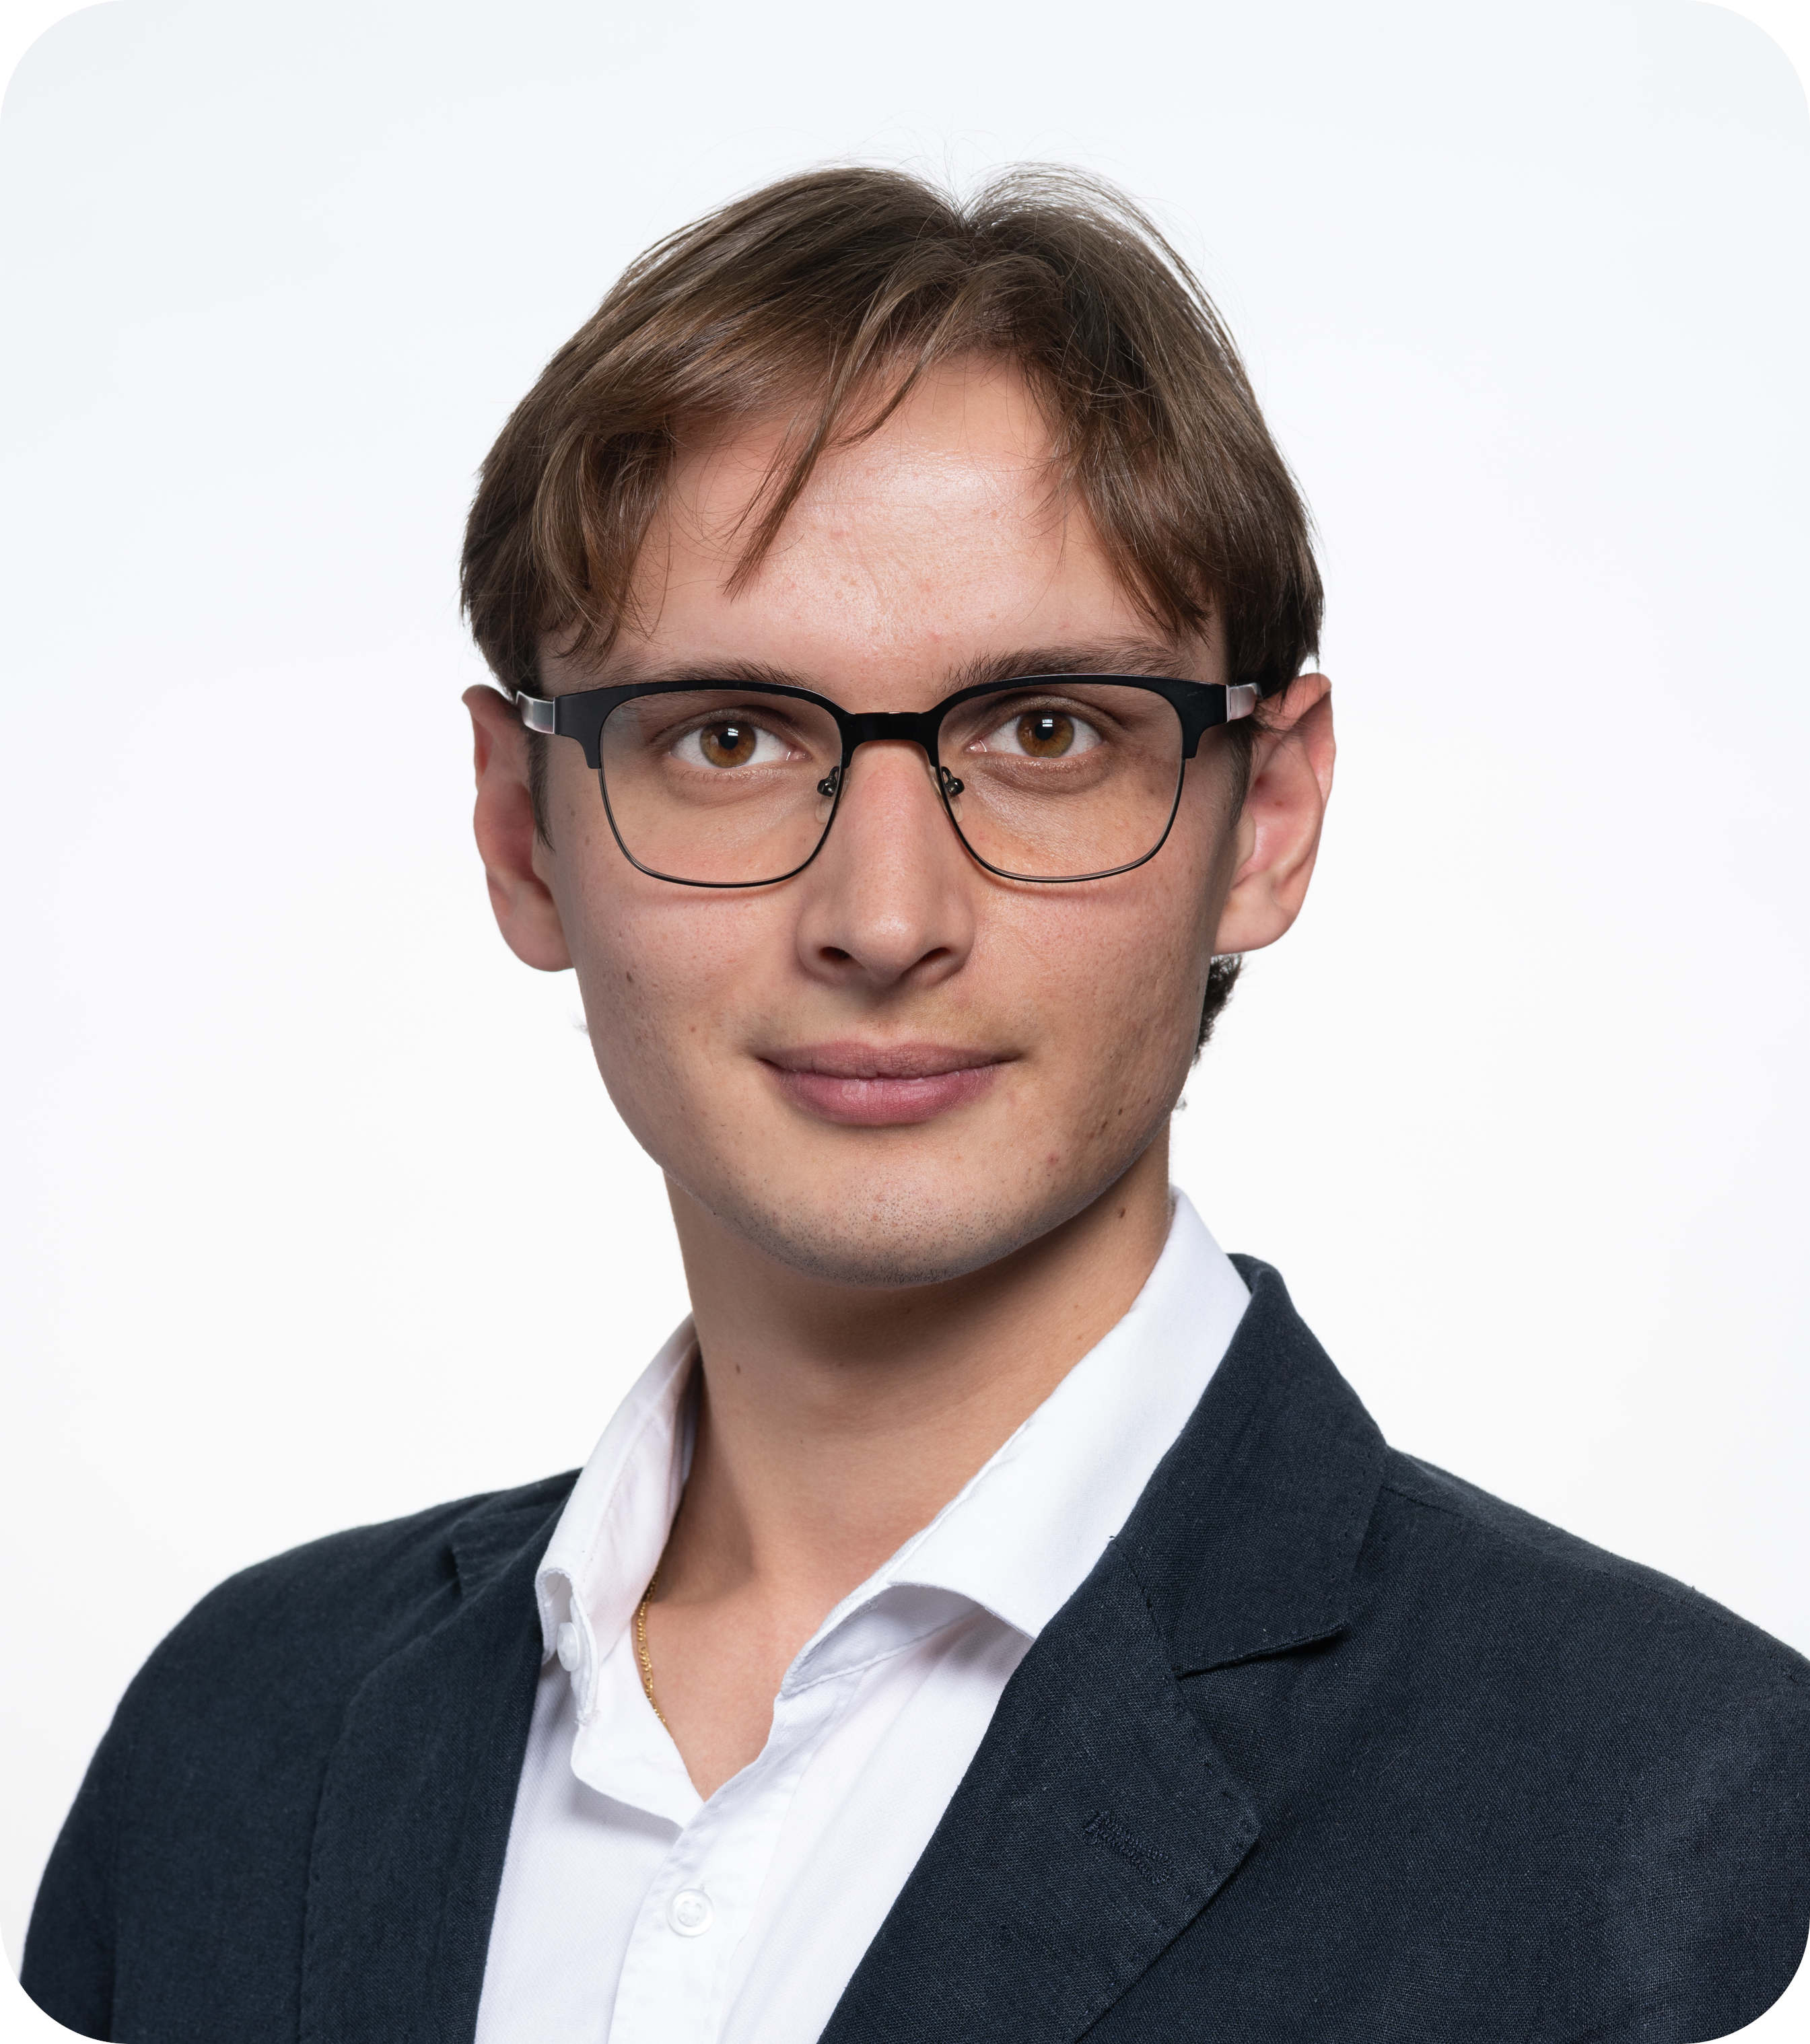
\includegraphics[width=\linewidth,keepaspectratio]{SquareLeoRound.jpg}%
  \end{minipage}%
  %\hspace{0.8em}% gap
  \hspace{1cm}
  % right: text block (top‑aligned + zero‑strut)
  \begin{minipage}[t]{\dimexpr\linewidth-3cm-0.8em\relax}%
    \vspace{0pt}% ← key: sets baseline at the very top
    %\centering
}{%
  \end{minipage}%
  % tighten space below header
  \vspace*{-0.2cm}%
}

% Last‐updated text
\newcommand{\placelastupdatedtext}{%
  \AddToShipoutPictureFG*{%
    \put(
        \LenToUnit{\paperwidth-2 cm-0.2 cm+0.05cm},
        \LenToUnit{\paperheight-1.0 cm}
    ){\vtop{{\null}\makebox[0pt][c]{
        \small\color{gray}\textit{Last updated April 2025}\hspace{\widthof{Last updated April 2025}}
    }}}%
  }%
}

% Link arrow
\let\hrefWithoutArrow\href
\renewcommand{\href}[2]{%
  \hrefWithoutArrow{#1}{\ifthenelse{\equal{#2}{}}{}{#2 }\raisebox{.15ex}{\footnotesize \faExternalLink*}}%
}

\begin{document}
    \newcommand{\AND}{\unskip
        \cleaders\copy\ANDbox\hskip\wd\ANDbox
        \ignorespaces
    }
    \newsavebox\ANDbox
    \sbox\ANDbox{}

    %\placelastupdatedtext
    \begin{header}
        \fontsize{30 pt}{30 pt}\textnormal{Leonardo Silvagni}
        \vspace{0.1 cm}

        \fontsize{16 pt}{16 pt}\textnormal{Neuro Engineering student at EPFL}
        
        \normalsize
        \vspace{0.1cm}
        \mbox{{\footnotesize\faMapMarker*}\hspace*{0.13cm}1023, Crissier, Switzerland}%
        \kern 0.25 cm\AND%
        \mbox{\hrefWithoutArrow{mailto:leonardo.silvagni@gmail.com}{{\footnotesize\faEnvelope[regular]}\hspace*{0.13cm}leonardo.silvagni@gmail.com}}%
        \kern 0.25 cm\AND%
        \mbox{\hrefWithoutArrow{tel:+41783169108}{{\footnotesize\faPhone*}\hspace*{0.13cm}+41 78 316 9108}}%
        \kern 0.25 cm\AND%
        \mbox{\hrefWithoutArrow{https://www.linkedin.com/in/leonardo-silvagni}{{\footnotesize\faLinkedinIn}\hspace*{0.13cm}linkedin.com/in/leonardo-silvagni}}%
    \end{header}

    \vspace{0.1 cm}

    \section{Profile}
    \begin{onecolentry}
        \textbf{Key strengths:} Signal Processing, Machine Learning, Electronics.\\
        %Biomedical engineer by training and interested in interfacing with the nervous system. 
        %Experienced in data manipulation, statistical analysis, and machine learning. Proficient in Python, R, Matlab, C/C++, and skilled in tools such as Torch, Pandas, Numpy, Scipy, git, LaTeX as well as image and signal processing, computer vision, neural data such as EEG, EMG and fMRI.
    \end{onecolentry}
    \section{Education}

    \begin{threecolentry}{\textbf{MSc}}{2024-Present}{\textbf{EPFL École Polytechnique Fédérale de Lausanne}, Neuro Engineering}
    \end{threecolentry}
    \vspace{0.2 cm}
    \begin{threecolentry}{\textbf{BSc}}{2024}{\textbf{ETSIT Politécnica de Madrid}, Biomedical Engineering. (Erasmus)}
    \end{threecolentry}
    \vspace{0.2 cm}
    \begin{threecolentry}{\textbf{BSc}}{2021-2024}{\textbf{University of Padova}, Biomedical Engineering.\\Final mark: 110 Cum Laude/110}
    
    \end{threecolentry}

    \section{Projects and Research}
    \begin{comment}
    \begin{twocolentry}{2025\\EPFL, Lausanne
    }
        \textbf{Development of a protocol to treat upper limb spasticity via peripheral nerve stimulation}
        \begin{highlights}
        \end{highlights}
    \end{twocolentry}

    \vspace{0.2 cm}
    \end{comment}


    \begin{twocolentry}{2025\\Personal Project
    }
        \textbf{Haptic Gait Guidance System for Obstacle Detection via Stereo Vision and Inertial Sensing (in progress)}
        \begin{highlights}
            \item Focus: embedded computer vision algorithms, sensor fusion (IMU and cameras), energy optimization.
        \end{highlights}
    \end{twocolentry}
    
    \begin{twocolentry}{2025\\EPFL, Lausanne, CH
    }
        \textbf{Extended Gate Transistor for biosensing application (in progress)}
        \begin{highlights}
            \item Reworked (CAD) previous design to reduce parasitic capacitance by 45\%, to improve limit of detection.
            \item Fabrication and testing of the devices. (cleanroom and wet/dry lab)
        \end{highlights}
    \end{twocolentry}
    \begin{comment}
    \begin{twocolentry}{2025\\EPFL, Lausanne, CH
    }
        \textbf{Hybrid computational model of epidural spinal cord stimulation}
        \begin{highlights}
            \item Built a hybrid modeling framework integrating FEM-based electromagnetic simulations with a spinal cord biophysical model to optimize gait rehabilitation outcomes.
            \item Reduced previous pipeline runtime 12 fold
        \end{highlights}
    \end{twocolentry}
    \end{comment}
    \vspace{0.2 cm}
    \begin{twocolentry}{2024\\EPFL, Lausanne, CH
        }
        \href{https://github.com/fedemengo/CS-433-ML4S}{\textbf{Machine Learning: Task prediction using fMRI data.}}
        \begin{highlights}
            \item Developed and validated Recurrent Neural Network models to deconvolve the timecourses of task paradigms from brain imaging data (fMRI) from the Human Connectome Project's task-based dataset.
        \end{highlights}
    \end{twocolentry}

    \vspace{0.2 cm}

    \begin{twocolentry}{2024\\ETSIT, Madrid, ES
    }
        \textbf{Development of an ESP32 based oxypulsimeter}
        \begin{highlights}
            \item Implemented embedded real time signal processing to extract heart rate and blood oxygen saturation from the PPG signal.

        \end{highlights}
    \end{twocolentry}
    \vspace{0.2cm}

    
    \begin{twocolentry}{2023-2024\\UNIPD, Padova, IT
    }
        \href{https://hdl.handle.net/20.500.12608/68828}{\textbf{Dynamic Bayesian Models of progression in Amyotrophic Lateral Sclerosis}}
        \begin{highlights}
            \item Validated an existing model in the scope of \textit{Explainable AI} for clinical data, using Dynamic Bayesian Networks.
        \end{highlights}
    \end{twocolentry}
    \vspace{0.2 cm}
    \begin{comment}

    \begin{twocolentry}{2024\\EPFL, Lausanne
    }
        \textbf{Temporal Interference Stimulation and concurrent EEG recording}
        \begin{highlights}
            \item Development of a motor learning paradigm.
        \end{highlights}
    \end{twocolentry}

    \vspace{0.2 cm}
    \end{comment}
    
    
    
    \begin{comment}
    \begin{twocolentry}{
    }
        \textbf{Neuromuscular model of zebrafish movement using Dynamical Systems theory}
        \begin{highlights}
        \end{highlights}
    \end{twocolentry}

    \vspace{0.2 cm}
    \end{comment}


    \section{Technical Skills}
    \begin{onecolentry}
      \textbf{Programming Languages:} Python, R, Matlab, C/C++, LaTeX
    \end{onecolentry}
    \vspace{0.1 cm}
    
    \begin{onecolentry}
      \textbf{Tools:} git, Torch, Pandas, Numpy, Scipy, OpenCV, Scikit-learn
    \end{onecolentry} 
    \vspace{0.1 cm}    


    \begin{onecolentry}
      \textbf{Skills:} Machine Learning, Electronics, CAD, Image and signal processing, FEM/COMSOL, Computer Vision, Microfabrication, Statistical Analysis
    \end{onecolentry} 



    \section{Work Experiences}

    \begin{twocolentry}{
        Arzignano, VI, IT

2018 - 2020
    }
        \textbf{Electronics Teacher}, Library Giulio Bedeschi
        \begin{highlights}
            \item Taught introductory courses on the Arduino platform and basic electronics to 20 students aged 13-18.
            \item Guided 25 students aged 12-16 in robotics challenges for the First Lego League competition. Team placed 4th on national level.
          \end{highlights}
    \end{twocolentry}

    \vspace{0.2 cm}    
    \begin{twocolentry}{
        Padova, IT

2021 - 2024
    }
        \textbf{Tutoring and teaching assistant},  University of Padova
        \begin{highlights}
            \item Peer tutored university students on the courses of \textit{Control systems, Electronics, Linear Algebra, Physics (classical and electromagnetism), Calculus I \& II}
          \end{highlights}
    \end{twocolentry}
    \vspace{0.2 cm}

\begin{comment}
    \section{Conferences \& Meetings}

    \begin{twocolentry}{
        Bologna, IT

        2024
    }
        \textbf{\href{https://boost24.elicsir.it/}{BOOST24}}, Elicsir Foundation
        \begin{highlights}
            \item Summer school (10 days) focused on machine learning, computation, graph theory, cloud, bioinformatics, and history of the field.
        \end{highlights}
    \end{twocolentry}

    \vspace{0.2 cm}

    \begin{twocolentry}{2023 - 2025}{
        \textbf{\href{https://www.gtec.at/spring-school-2024/}{BCI and Neurotechnology Spring Schools} and Masterclasses}, g.tec medical engineering GmbH
        \begin{highlights}
          \item Spring schools (140 hours) on BCI and neurotechnology with a focus on the latest advancements in the field.
      \end{highlights}
      }
      \end{twocolentry}

    \vspace{0.2 cm}

    \begin{twocolentry}{
        Rieti, IT

2023
    }{
        \href{https://fa23.bici.events/}{\textbf{Futuro Annunciato}}, Elicsir Foundation
        \begin{highlights}
            \item Summer school (3 days) on informatics with events from academia, industry, and startups.
        \end{highlights}
    }
    \end{twocolentry}
\end{comment}
    \section{Organizations}

    \begin{twocolentry}
        {2024 - 2025}{\textbf{Lead The Future Mentorship}\\  
        Mentorship program for Italian STEM students.}
    \end{twocolentry}

    \vspace{0.1 cm}

    \begin{twocolentry}
        {2023}{\textbf{Bioleap}, Nucleate Italy\\
        Informative program of 4 months about medtech and startups.}
    \end{twocolentry}

    \section{Recognitions \& Awards}

    \begin{threecolentry}
        {2025}{Harvard, Boston, USA}{\textbf{Bertarelli Harvard EPFL Fellowship}\\
        %Awarded 45.000\$ grant and paid tuition fee to conduct my master thesis at Harvard Medical School.
        Awarded a 120 000 \$ fellowship (75 000 \$ tuition + 45 000 \$ research and living expenses) for a master thesis at Harvard Medical School.
        }
    \end{threecolentry}

    \vspace{0.1 cm}

    \begin{threecolentry}
        {2023}{University of Padova, IT}{\textbf{Mille ed una lode Scholarship}  \\
        Scholarship based on merit given to approximately the top 3\% of each class.}
    \end{threecolentry}
    \vspace{0.1 cm}
    \begin{threecolentry}
        {2023-2024}{Elicsir foundation, Bologna, IT}{\textbf{\href{https://boost24.elicsir.it/}{Summer Schools}}  \\
        Scholarships to attend a 10 days and a 4 days summer school with focus on machine learning, computation, cloud, bioinformatics and history of informatics.}
    \end{threecolentry}
    \vspace{0.1cm}
    \begin{threecolentry}
        {2021-2024}{University of Padova, IT}{\textbf{STEM degrees incentives}  \\
        Scholarship based on merit.}
    \end{threecolentry}


    \section{Languages}

    \begin{onecolentry}
        \textbf{English:}  C1 (TOEFL 112) \\
        \textbf{Italian:}  C2   \\
        \textbf{French:}  A2/B1 (aim to acheive B1/B2 by early 2026) \\
        \textbf{Spanish:}  B1\\
    \end{onecolentry}
    
    \section{Information}

    \begin{onecolentry}
        \textbf{Work permit:} B (Switzerland) \\
        \textbf{Driving license:} Yes  \\
    \end{onecolentry}


    
    \section{Extracurriculars}

    \begin{onecolentry}
            Vice President and sponsoring contact for Neuro Engineering student association at EPFL (2024-2025). \\Alpine Club of Italy (CAI) youth guide, parish summer-camp organizer, blood donor, IEEE member. \\ 
        Enjoy hiking and mountaineering in my free time.
    \end{onecolentry}
    \vspace{\fill}
    Lausanne, \today

    \section{Personal Data}
    \begin{onecolentry}
        I hereby authorize the use of my personal data in accordance with GDPR 679/16.
    \end{onecolentry}

\end{document}
